% Преамбула

% определяем формат страницы и тип документа ( А4, 12 пунктов, статья)
\documentclass[a4paper,12pt]{article}

% Задаём отступы и межстрочный интервал
\usepackage[top=2cm,bottom=2cm,left=3cm,right=2cm,marginparwidth=1.75cm]{geometry}

% подключаем пакеты расширения LaTeX
\usepackage{cmap}					% поиск в PDF
\usepackage[T2A]{fontenc}			% кодировка
\usepackage[utf8]{inputenc}			% кодировка исходного текста
\usepackage[english,russian]{babel}	% Русский язык и переносы
\usepackage{indentfirst} 			% красная строка
\frenchspacing						
\usepackage[utf8]{inputenc}			% кодировка	
\usepackage[T1]{fontenc}			

% полезные пакетики
\usepackage{amsmath} 									% для продвинутых формул
\usepackage{graphicx}									% для графиков
\usepackage[colorinlistoftodos]{todonotes}				% для пометок
\usepackage[colorlinks=true, allcolors=blue]{hyperref}	% расширенная поддержка гиперссылок
\usepackage{comment}									% многострочные комментарии
\usepackage{ulem}										% зачёркнутый текст
\usepackage{xcolor}										% цветной текст
\usepackage{color}										% цветной код
\usepackage{listings}									% отображает блоки кода

% настройка пакета подсветки исходного кода (не совсем рабочий)
\lstloadlanguages{ [LaTeX ] TeX, bash , Fortran , Perl ,C++,make} 
\lstset{ 			language =[LaTeX ] TeX,		 % выбираем язык по умолчанию
                    extendedchars=true , 		 % включаем не латиницу (не работает)
                    escapechar =| , 			 % |«выпадаем» в LATEX|
                    frame=tb , 					 % рамка сверху и снизу ( lr - слева, справа )
                    commentstyle=\itshape , 	 % шрифт для комментариев
                    stringstyle =\bfseries }	 % шрифт для строк



\author{ООО "ЛМП"} % Вводим своё имя
\title{Ошибка нерциальных датчиков МГ-25 в температуре}  % Заголовок
\date{\today} % установка даты

\begin{document}
\maketitle
% \begin{abstract}
% Your abstract.
% \end{abstract}

\section{Ошибки прибора МГ-25}
\subsection{Оценка ошибки смещения нуля при изменении температуры по шагам}
Были проведены эксперименты с охлаждением устройства МГ-25 до -40 градусов цельсия, при которых он находился 3 часа, затем производился нагрев с шагом в 20 градусов (точки -40, -20, 0, 20, 40, 60 и 80 градусов цельсия). В каждой температурной точке датчик сначала выдерживался на протяжении одного часа, а затем производились измерения в течение одной минуты. Сразу же после достяжения самой высокой температуры датчик был охлаждён по аналогичному алгоритму: в точках 70, 50, 30, 10, -10, и -30 градусов цельсия датчик сначала находился 1 час, затем снимались данные на протяжении 30 секунд. В каждой точке данные акселерометров и ДУС были усреднены и построены графики изменения смещения нуля в температуре. На рисунке ~\ref{fig:gyro_bias_steps} представлены графики смещения нуля датчиков угловой скорости в температуре. На рисунках ~\ref{fig:Ax_accel}, ~\ref{fig:Ay_accel} и ~\ref{fig:Az_accel} представлены графики смещения нуля акселерометров в температуре.

Изначально датчик был откалиброван в диапазоне температур от -20 до 85 $^o$C, из-за чего измерения в точках -40 и -30 $^o$C на некоторых графиках имеют уход и поэтому рассматриваться не будут.

В соответствии с графиком ~\ref{fig:gyro_bias_steps} максимальные отклонения угловой скорости в температуре для осей X,Y и Z составляют 20, 40 и  60 $^o$/ч соответственно.

В соответствии с графиками ~\ref{fig:Ax_accel},~\ref{fig:Ay_accel} и ~\ref{fig:Az_accel} максимальные отклонения от среднего значения в температуре для трёх осей X Y Z акселерометров составляют $\pm1.5$, $\pm0.2$ и  $\pm5$ mg  соответственно.


\begin{figure}[hp!]
\centering
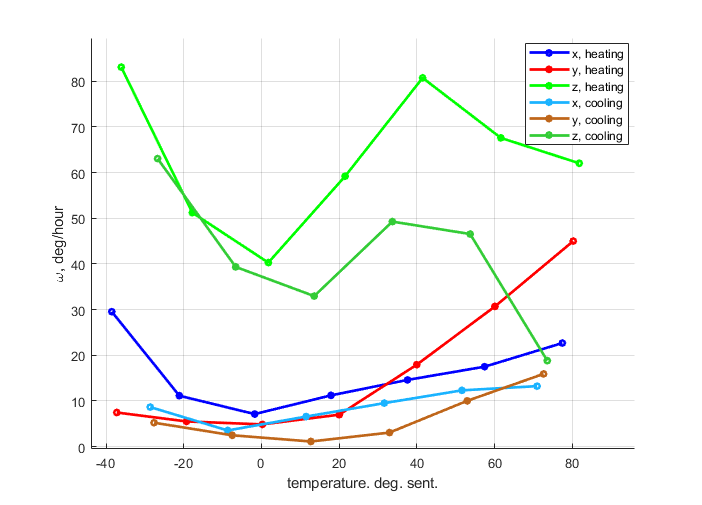
\includegraphics[width=0.9\textwidth]{gyro_bias_steps3.png}
\caption{\label{fig:gyro_bias_steps} Смещения нуля ДУС в температуре.}
\end{figure}
\begin{figure}[hp!]
\centering
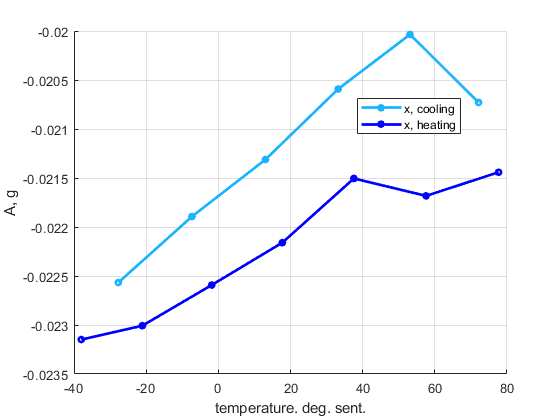
\includegraphics[width=0.9\textwidth]{Ax_accel.png} 
\caption{\label{fig:Ax_accel} Смещения нуля оси Х акселерометра в температуре.}
\end{figure}
\begin{figure}[hp!]
\centering
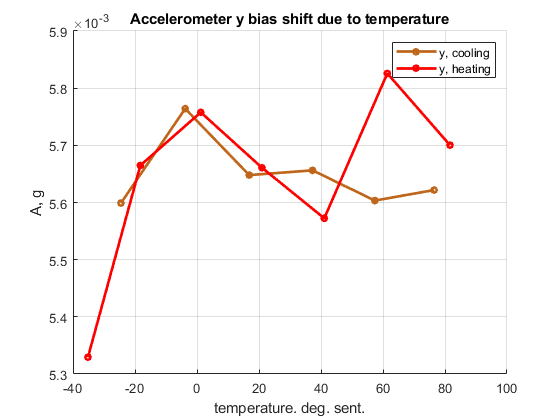
\includegraphics[width=0.9\textwidth]{Ay_accel.png} 
\caption{\label{fig:Ay_accel} Смещения нуля оси Y акселерометра в температуре.}
\end{figure}
\begin{figure}[hp!]
\centering
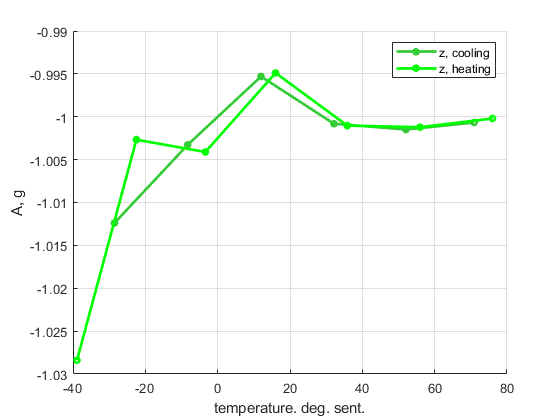
\includegraphics[width=0.9\textwidth]{Az_accel.png} 
\caption{\label{fig:Az_accel} Смещения нуля оси Z акселерометра в температуре.}
\end{figure}

\subsection{Оценка ошибки смещения нуля ДУС при непрерывном изменении температуры}
Были проведены измерения показаний ДУС при нескольких экспериментах нагрева с последующим охлаждением с разными скоростями изменения температуры. Полученные графики нагрева осей X, Y и Z и охлаждения осей X,Y и Z приведены на рисунках ~\ref{fig:continius_wx_up},~\ref{fig:continius_wy_up},~\ref{fig:continius_wz_up},~\ref{fig:continius_wx_down},~\ref{fig:continius_wy_down} и ~\ref{fig:continius_wz_down} соответственно. Легенда на графиках отображает максимальную скорость изменения температуры в ходе измерений (скорость нагрева максимальна вначале измерений и начинает экспоненциально уменьшатся после достижения 70 градусов цельсия, типичный график температур в ходе экспериментов представлен на рисунке ).

На рисунке ~\ref{fig:four_exps} представлены результаты измерения нагрева трёх осей при максимальных скоростях измененеия температуры 5.2-5.4 $^{\circ}$C/мин. Испытания проводились при различных положениях датчика, поэтому начальные значения могут различаться в пределах $\pm$15$^{\circ}$C/час вследствие влияния вращения земли.

На рисунке ~\ref{fig:hyst} представлен один из экспериментов охлаждения с последующим нагревом со скоростью нагрева  5.4 $^{\circ}$C/мин и скоростью охлаждения 2.5 $^{\circ}$C/мин. Как видно, на графике у всех осей есть значительный гистерезис. 

Анаогичный эксперимент, но с меньшим диапазоном температур представлен на рисунке ~\ref{fig:hyst_2}. Здесь датчик из точки 40 $^{\circ}$C нагрели до 60 $^{\circ}$C затем остудили до 20 $^{\circ}$C и затем снова нагрели до 40 $^{\circ}$C. Как видно из графика, гистерезис существенный, но не такой большой, как гистерезис на рисунке ~\ref{fig:hyst}.

% %%
\begin{figure}[h]
\centering
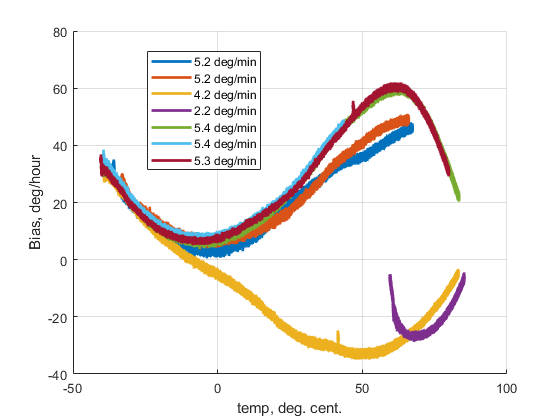
\includegraphics[width=0.9\textwidth]{continius_wx_up.png} 
\caption{\label{fig:continius_wx_up}Смещения нуля оси Х при различных скоростях измерения температуры. Нагрев.}
\end{figure}
%%
\begin{figure}[h]
\centering
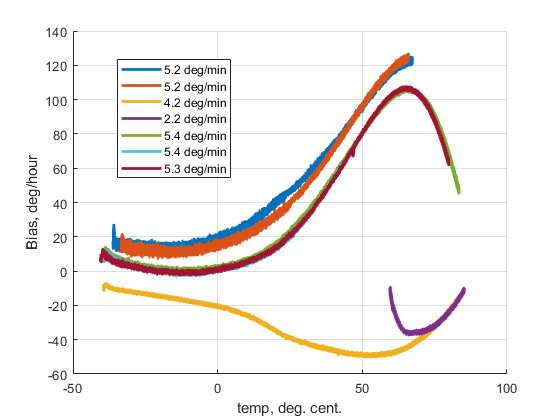
\includegraphics[width=0.9\textwidth]{continius_wy_up.png} 
\caption{\label{fig:continius_wy_up}Смещения нуля оси Y при различных скоростях измерения температуры. Нагрев.}
\end{figure}
%%
\begin{figure}[h]
\centering
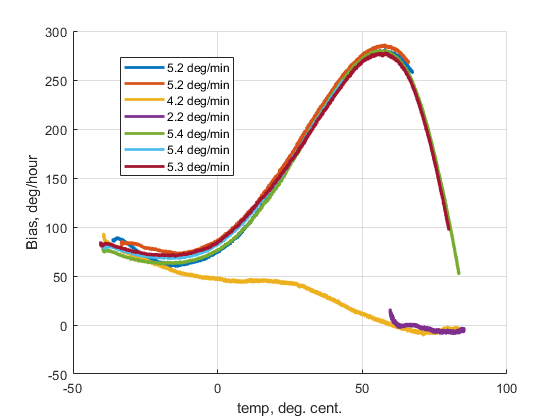
\includegraphics[width=0.9\textwidth]{continius_wz_up.png} 
\caption{\label{fig:continius_wz_up}Смещения нуля оси Z при различных скоростях измерения температуры. Нагрев.}
\end{figure}
%%
%%
\begin{figure}[h]
\centering
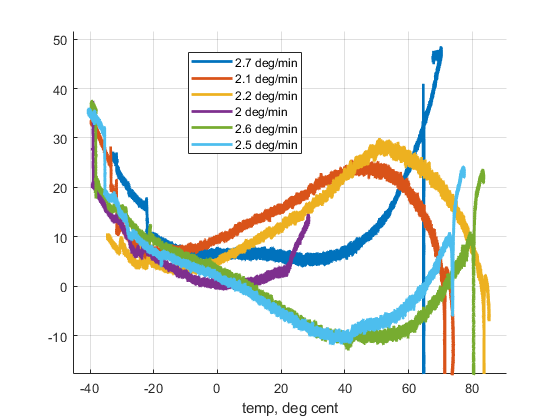
\includegraphics[width=0.9\textwidth]{continius_wx_down.png} 
\caption{\label{fig:continius_wx_down}Смещения нуля оси Х при различных скоростях измерения температуры. Охлаждение.}
\end{figure}
%%
\begin{figure}[h]
\centering
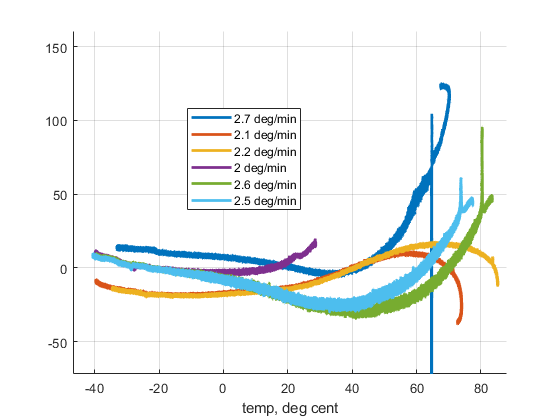
\includegraphics[width=0.9\textwidth]{continius_wy_down.png} 
\caption{\label{fig:continius_wy_down}Смещения нуля оси Y при различных скоростях измерения температуры. Охлаждение.}
\end{figure}
%%
\begin{figure}[h]
\centering
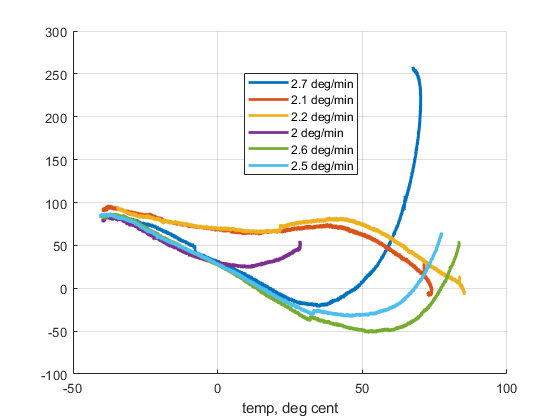
\includegraphics[width=0.9\textwidth]{continius_wz_down.png} 
\caption{\label{fig:continius_wz_down}Смещения нуля оси Z при различных скоростях измерения температуры. Охлаждение.}
\end{figure}

%%%%%%%%%%%%%%%


\begin{figure}[hp!]
\centering
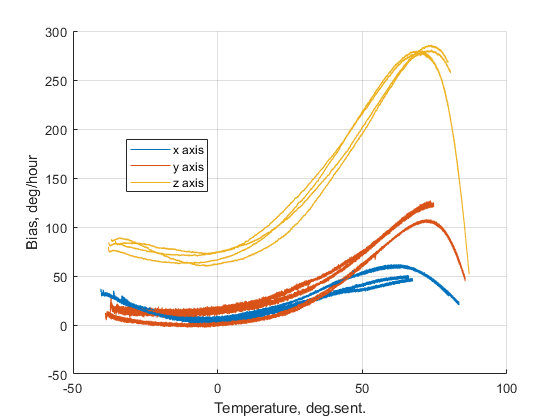
\includegraphics[width=0.9\textwidth]{four_graphs.png} 
\caption{\label{fig:four_exps} Смещения нуля ДУС при повышении температуры. Четыре эксперимента.}
\end{figure}
\begin{figure}[hp!]
\centering
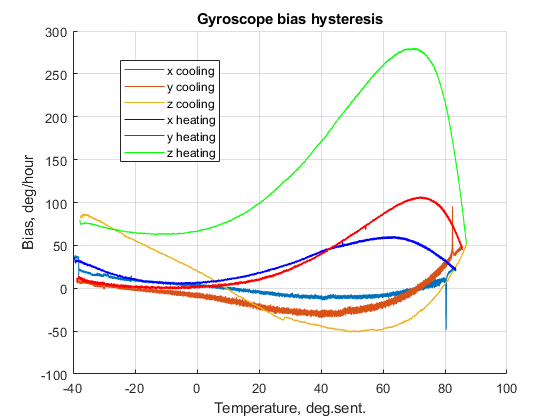
\includegraphics[width=0.9\textwidth]{hysteresis.png} 
\caption{\label{fig:hyst} Гистерезис угловой скорости. Нагрев сменяется охлаждением. Нагрев 5.4 $^{\circ}$C/мин, охлаждение 2.4 $^{\circ}$C/мин.}
\end{figure}

\begin{figure}[hp!]
\centering
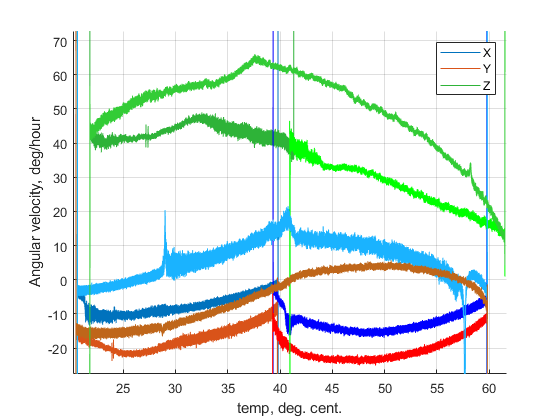
\includegraphics[width=0.9\textwidth]{circle.png} 
\caption{\label{fig:hyst_2} Термоцикл нагрев-охлаждение-нагрев. нагрев 1.8 $^{\circ}$C/мин, охлаждение 2.4 $^{\circ}$C/мин.}
\end{figure}

Для нахождения того, как быстро меняется смещения нуля за один градус цельсия, была посчитана производная от смещения нуля в температуре. Типичный график представлен на рисунке  ~\ref{fig:gradi}. Как видно из графиков, изменение смещения нуля может достигать 1-2 градусов в час на градус цельсия для осей $X$ и $Y$ и 4 градусов в час на градус цельсия для  оси $Z$.

\begin{figure}[hp!]
\centering
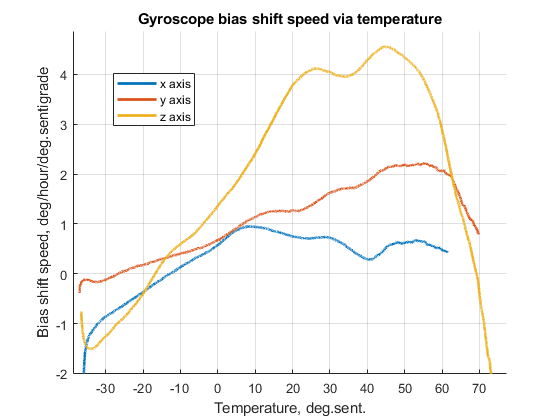
\includegraphics[width=0.9\textwidth]{gradient_labeled.png} 
\caption{\label{fig:gradi} Изменения смещения нуля ДУС за один градус цельсия от температуры, $^{\circ}/h/^{\circ}C$ (см. комментарии к рисунку на стр. Х).}
\end{figure}

На рисунках ~\ref{fig:accX_hyst} и ~\ref{fig:accY_hyst} приведены графики смещения нулей в температуре для осей $X$ и $Y$ акселерометра. 

В соответствии с графиком ~\ref{fig:hyst}, максимальные отклонения угловой скорости на всём диапазоне температур составляют 70, 120 и 310 $^{\circ}$/час для осей X,Y и Z соответственно. Для диапазона от 20 до 60  $^{\circ}$С (рис ~\ref{fig:accX_hyst_2}) ошибки составляют 30, 34 и 52 $^{\circ}$/час для осей X,Y и Z соответственно.
\begin{figure}[hp!]
\centering
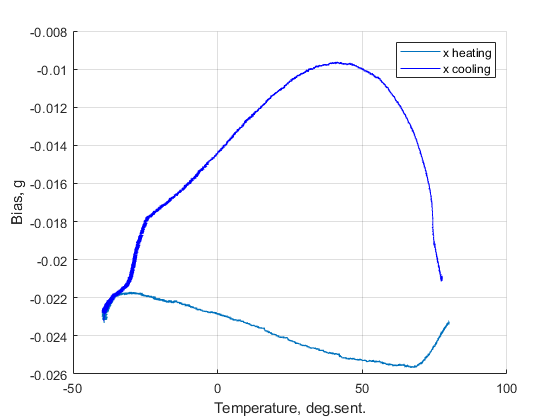
\includegraphics[width=0.9\textwidth]{AccX_hyst.png} 
\caption{\label{fig:accX_hyst} Смещение нуля в температуре. Акселерометр. Ось Х.}
\end{figure}

\begin{figure}[hp!]
\centering
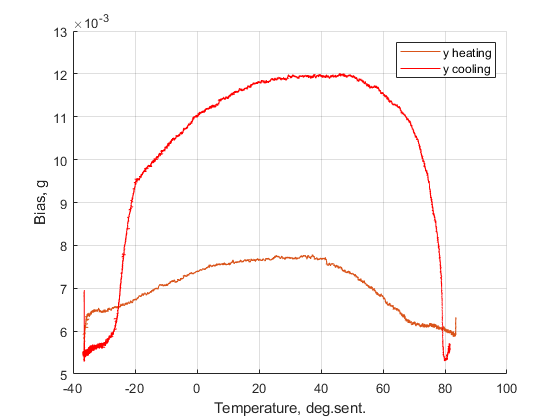
\includegraphics[width=0.9\textwidth]{AccY_hyst.png} 
\caption{\label{fig:accY_hyst}  Смещение нуля в температуре. Акселерометр. Ось Y.}
\end{figure}

%%
\begin{figure}[hp!]
\centering
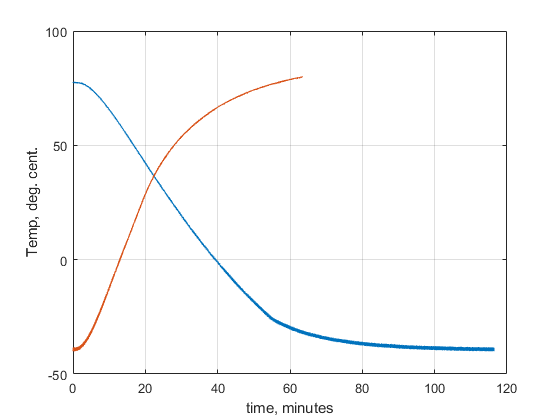
\includegraphics[width=0.9\textwidth]{temp_typical.png} 
\caption{\label{fig:temp_typical}  Типичный график изменения температур во время экспериментов. Нагрев и охлаждение.}
\end{figure}
%%


\subsection{Оценка ошибки смещения нуля и масштабного коэффициента на одной температурой точке на поворотном столе}
Для оценки ошибок смещения нуля акселерометров и ДУС прибор МГ-25 был повёрнут в 26 различных положений на поворотном столе. В каждом положении по показаниям поворотного стола были вычислены истинные ускорения и угловые скорости, которые затем были вычтены из действительных показаний прибора МГ-25, приведённых к координатам поворотного стола. Получившиеся смещения нуля акселерометра показаны на рисунке  ~\ref{fig:accel_biases}.

\begin{figure}[hp!]
\centering
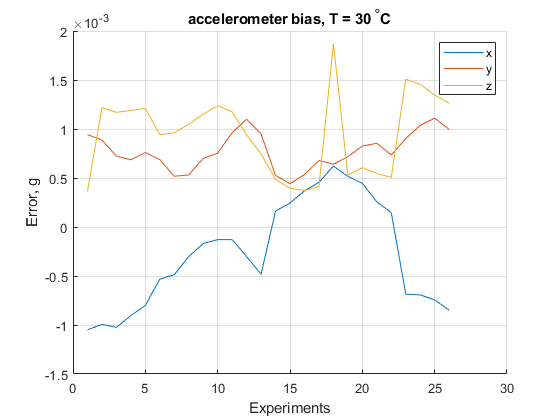
\includegraphics[width=0.9\textwidth]{accel_biases.png} 
\caption{\label{fig:accel_biases}  Смещение нуля акселерометра в разных положениях.}
\end{figure}

Матрица приведения данных МГ-25 к базису поворотного стола находилась следующим образом: усреднённые данные акселерометров с трёх положений (ось Х вверх, ось Y вверх, ось Z вверх) составляли матрицу измеренных значений $A$, при этом матрица истинных значений $B$ известна. При помощи методов оптимизации решалась задача нахождения такой матрицы $\widetilde{A} = RS(B-b)$, что модуль разницы $|A-\widetilde{A}|$ был минимальным. Здесь $R$ - ортонормированная матрица приведения данных, $S$ - диагональная матрица с масштабными коэффициентами, близкими к единице, $b$ -  матрица смещений нуля акселерометров для соответствующих осей. 

После нахождения матрицы приведения, масшабные коэффициенты для акселерометров и смещения нулей получились следующими: $S = \begin{bmatrix} 1.00002 \\ 0.99993 \\1.0003 \end{bmatrix}$  и $b = \begin{bmatrix}  0.0002\\  0.0008\\ -0.0009 \end{bmatrix} g$
. 



Полученные ошибки гироскопов после применения матрицы доворота представлены на рисунке ~\ref{fig:gyros_errors}. Здесь фиолетовым графиком отображён модуль угловой скорости, которой подвергался датчик. Ось значений расположена справа от графика.

Аналогично акселерометрам, масштабные коэффициенты ДУС и смещения нулей получились следующими: $S = \begin{bmatrix} 1.0008 \\ 1.001 \\ 1.0001\end{bmatrix}$ и $b = \begin{bmatrix}  -0.017 \\ -0.004\\ -0.01\end{bmatrix}$ $^{\circ}$/c. 
% Для датчиков угловой скорости были проведены аналогичные эксперименты: 26 статических положений, 26 положений при вращении внешней оси поворотника со скоростью 30 $^{\circ}$/с и по 4 положения с вращением вокруг оси $Z$ со скоростями $\pm$60, $\pm$120 и $\pm$180 $^{\circ}$/с. Полученные результаты показаны на рисунке ~\ref{fig:gyros_errors}. Из-за не идеальности калибровки на скоростях $\pm$60, $\pm$120 и $\pm$180 30 $^{\circ}$/с ось $Y$ измеряет значительную проекцию вращения.

\begin{figure}[hp!]
\centering
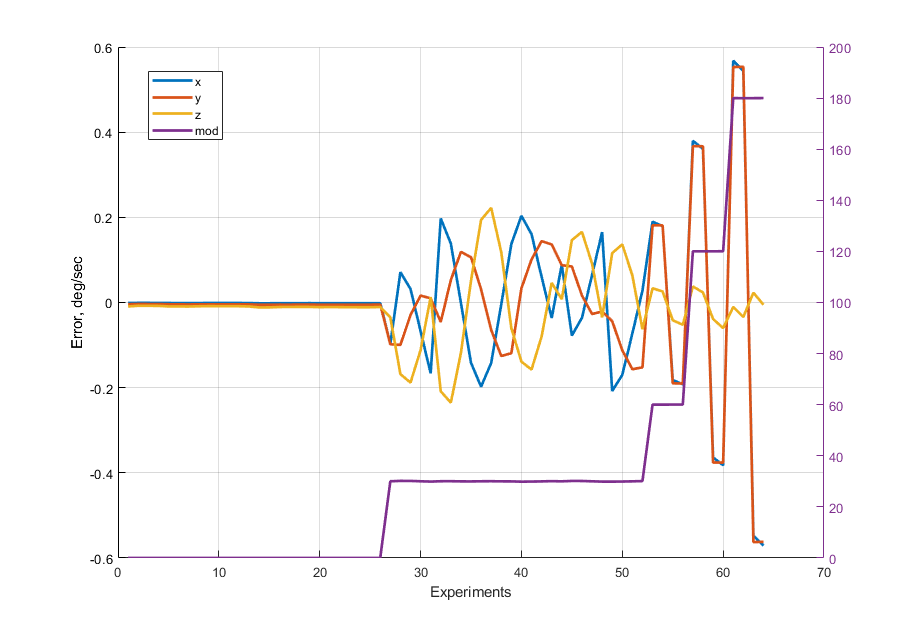
\includegraphics[width=0.9\textwidth]{velocity_errors.png} 
\caption{\label{fig:gyros_errors}  Смещение нуля ДУС в разных положениях. Справа (фиолетовым) показана угловая скорость, которую испытывал прибор.}
\end{figure}

% \begin{figure}[hp!]
% \centering
% 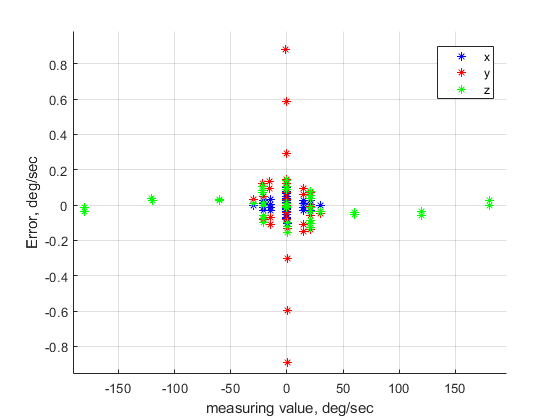
\includegraphics[width=0.9\textwidth]{gyros_errors_dots.png} 
% \caption{\label{fig:gyros_errors_dots}   Смещение нуля ДУС от измеренного осью ускорения.}
% \end{figure}



\section{Гирокомпасирование}
В данной работе под "углом места" подразумевается угол между осью Z прибора МГ-25 и вертикальной осью. То есть, если угол места равен 90 градусам, это означает, что датчик расположен горизонтально.
\subsection{Приведение системы координат МГ-25 к оси вращения.}

Для правильной работы алгоритма требуется привести оси (акселерометров и ДУС) к внутренней оси вращения системы. Для этого требуется поставить прибор МГ-25 в вертикальное положение (ось Z акселерометра вверх) и провести следующие процедуры: снять и усреднить показания акселерометра по оси $x$ (обозначим как $ax_1$) и y (обозначим как $ay_1$) в течение нескольких секунд, затем повернуть МГ-25 на 180 градусов внутренним двигателем и таким же образом ещё раз снять усреднённые показания осей х и у ($ax_2$ и $ay_2$).   \textcolor{red}{ Важно, чтобы остальная конструкция системы оставалась неподвижной во время всей процедуры.}



Для нахождения матрицы доворота используются следующие выражения\footnote{Для малых углов отклонения системы от вертикали (не более 7 градусов) можно использовать упрощенные формулы нахождения углов: $\alpha = \frac{ax_1+ax_2}{2}$ и $\beta = - \frac{ay_1+ay_2}{2}$, которые дадут дополнительную ошибку определения угла места не более 0.01 градуса. }:

\[ \alpha = \frac{arcsin(ax_1)+arcsin(ax_2)}{2}\]
\[ \beta = - \frac{arcsin(ay_1)+arcsin(ay_2)}{2}\]

\[
R = 
\begin{bmatrix}
cos(\alpha) & 0 & -sin(\alpha)\\
sin(\alpha)sin(\beta) & cos(\beta) & cos(\alpha)sin(\beta) \\
cos(\beta)sin(\alpha) & -sin(\beta) & cos(\alpha)cos(\beta)
\end{bmatrix}
\]

Если используется MatLab, $R = angle2dcm(0, \alpha, \beta)$.

Все получаемые в дальнейшем значения акселерометров и ДУС нужно предварительно домножить на матрицу $R$

\subsection{Проведенные эксперименты и результаты.}

Для исследования точности определения азимута прибором МГ-25, он был закреплён на трехосевом поворотном столе, внешняя ось поворотного стола задавала истинный угол азимута, вторая ось поворотного стола задавала угол места, третья ось - четыре поворота вокруг оси $Z$ прибора с шагом 90 градусов. Всего было снято 25 различных положений с разными углами азимута и места (Азимут - 0, 12, 90, 180 и 270 относительно севера, угол места - 1, 10, 20, 34, 56 градусов относительно вертикали). Эксперименты были проведены в комнатной температуре с предварительным ожиданием стабилизации температуры в приборе. В каждой точке, ипользуя показания акселерометров, вычисляется угол места прибора и затем по полученной проекции вектора вращения земли и вектора ускорения свободного падения на плоскость $XY$ датчика вычисляется угол азимута. В каждом положении датчик снимал показания 2 минуты за оборот (по 30 секунд на каждый оборот внутренней оси 0, 90, 180 И 270 градусов). Весь эксперимент был повторён 4 раза подряд для каждого положения, полученные ошибки усреднены по четырем точкам.   Во время четырёх поворотов оси $Z$ на 90 градусов записывались все данные с осей Х и Y гироскопа, однако для имитации вращения на 180 градусов в дальнейшем анализе данные делили на 4 поворота (4 точки съёма данных с поворотом 90 градусов) и 2 поворота (2 точки съёма данных с поворотом осей Х и Y на 180 градусов).

Зная истинное положение датчика по поворотному столу и получая значения угла места и азимута от прибора МГ-25 мы можем получить ошибки определения угла места и азимута. Типичный график ошибок для проведенных экспериментов представлен на рисунках ~\ref{fig:Azim} (\footnote{В каждом положении мы вращаем датчик на 90 градусов, тем самым снимая показания двумя осями Х и У со всех четырёх сторон и находим по ним угол азимута. Однако, в реальных условиях иногда возможно вращать прибор только на 180 градусов. Для вычисления азимута в этом случае используется одна часть данных с оси Х и другая часть данных с перпендикулярной оси У. Таким образом мы имеем все направления и можем вычислить проекцию вектора угловой скорости земли только по одному повороту на 180 при помощи двух осей. Из-за большего числа поворотов в ходе эксперимента мы можем комбинировать оси Х и У двумя способами, что и отображено на графике. }) и ~\ref{fig:Elev} . По оси х отложены разные положения прибора, упорядоченные по уменьшению угла места (у первых пяти точек угол места равняется 56 градусам, у последних - 1 градусу).

\begin{figure}[h!] 
\centering
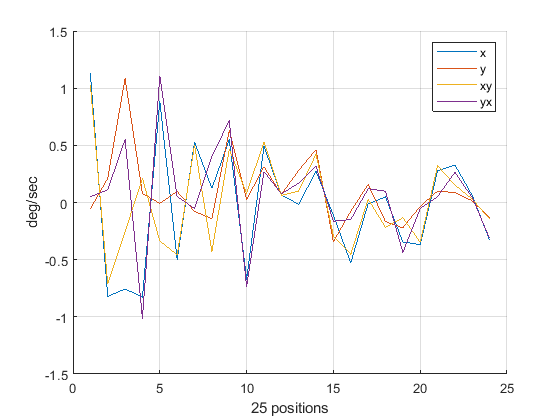
\includegraphics[width=0.9\textwidth]{Azim_err.png} 
\caption{\label{fig:Azim} Ошибка нахождения угла азимута (см. сноску 2).}
\end{figure}

\begin{figure}[h!] 
\centering
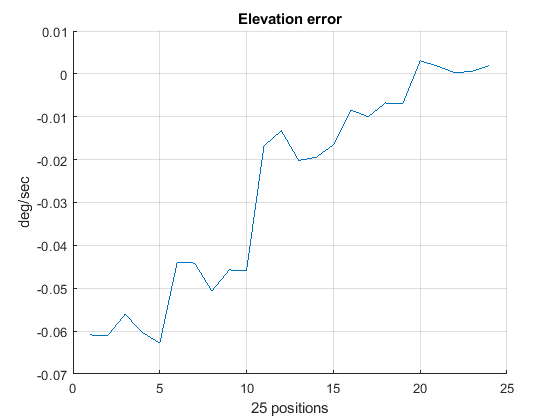
\includegraphics[width=0.9\textwidth]{Elev_err.png} 
\caption{\label{fig:Elev} Ошибка нахождения угла места (см. описание на странице 8).}
\end{figure}

Было проведено исследование влияния количества измерений и длительности одного измерения на ошибку нахождения угла азимута.  Исходные данные (4 повторения эксперимента с 4-мя поворотами на 90 градусов каждой оси с ожиданием в 30 секунд в каждой точке) были разделены по 10,20 и 30 секунд ожидания в каждой точке и усреднением результатов по 1,2,3 или 4 повторениям (рис ~\ref{fig:Matrix}, красным помечено общее время, необходимое для измерения).  Для каждой точки в получившейся сетке были посчитаны ошибки нахождения угла азимута и построены поверхности ошибок по исходной сетке. Пример поверхности для максимальной ошибки оси Х представлен на рисунке ~\ref{fig:Mesh}. 
\begin{table}[h]

\begin{center}
\begin{tabular}{ c | c | c | c }

   & 30 & 20 & 10 \\  \hline
 1 & 120 & 80 &  40\\  
 2 & 240 & 160 & 80\\  
 3 & 360 & 240 & 120\\
 4 & 480 & 320 & 160
\end{tabular}
\end{center}
\caption{\label{fig:Matrix}Сетка затраченного времени измерения в зависимости от времени и количества точек (слева - количество точек усреднения, сверху - время измерения в одной точке).}
\end{table}

% \begin{figure}[h!] 
% \centering
% 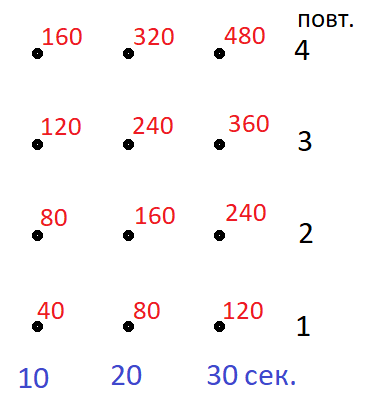
\includegraphics[width=0.4\textwidth]{matrix.png} 
% \caption{\label{fig:Matrix} Исходная сетка.}
% \end{figure}


\begin{figure}[h!] 
\centering
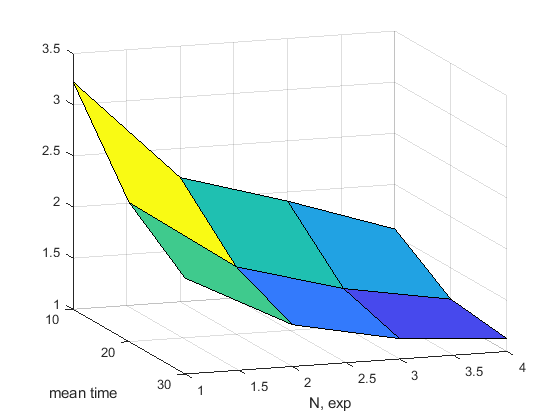
\includegraphics[width=0.9\textwidth]{mesh.png} 
\caption{\label{fig:Mesh} Максимальная ошибка оси Х.}
\end{figure}


Целью построения таких поверхностей было определение оптимальной стратегии измерения угла азимута - лучше ли за определённое время делать больше измерений, либо же просто дольше ждать и усреднять по большему интервалу времени. Из полученных графиков следует, что при стабильной температуре внутри прибора \textbf{нет разницы} между тем, каким образом вести измерения, точность измерения зависит лишь от самого общего времени, затраченного на измерения. Далее приведен график максимальной (~\ref{fig:err_max}) ошибки измерения угла азимута от времени, затраченного на измерения. 

 Из того, что в условиях неизменной температуры выбор пути проведения измерений не влияет на точность измерения угла места следует, что в реальных условиях (с нестабильной температурой) следует уменьшить время измерения в одном положении и увеличить общее количество измерений для минимизации влияния температуры на результат.

\begin{figure}[h!] 
\centering
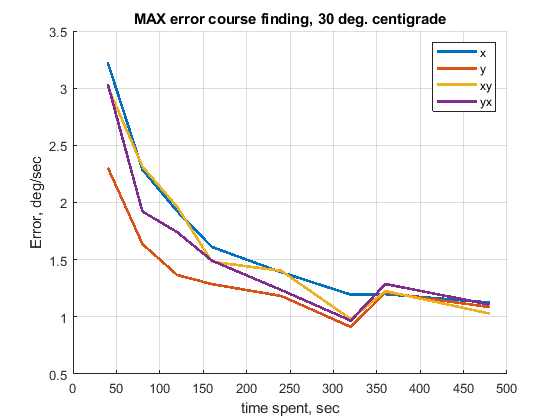
\includegraphics[width=0.9\textwidth]{err_max.png} 
\caption{\label{fig:err_max} Максимальная ошибка определения угла азимута от времени.}
\end{figure}

% \begin{figure}[h!] 
% \centering
% 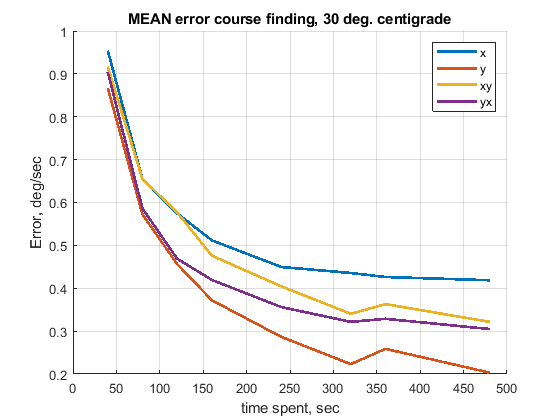
\includegraphics[width=0.9\textwidth]{mean_err.png} 
% \caption{\label{fig:err_mean} Средняя ошибка определения угла азимута от времени ().}
% \end{figure}




\end{document}